\chapter{Execute Stage}

\begin{figure}[H]   
	\centering
	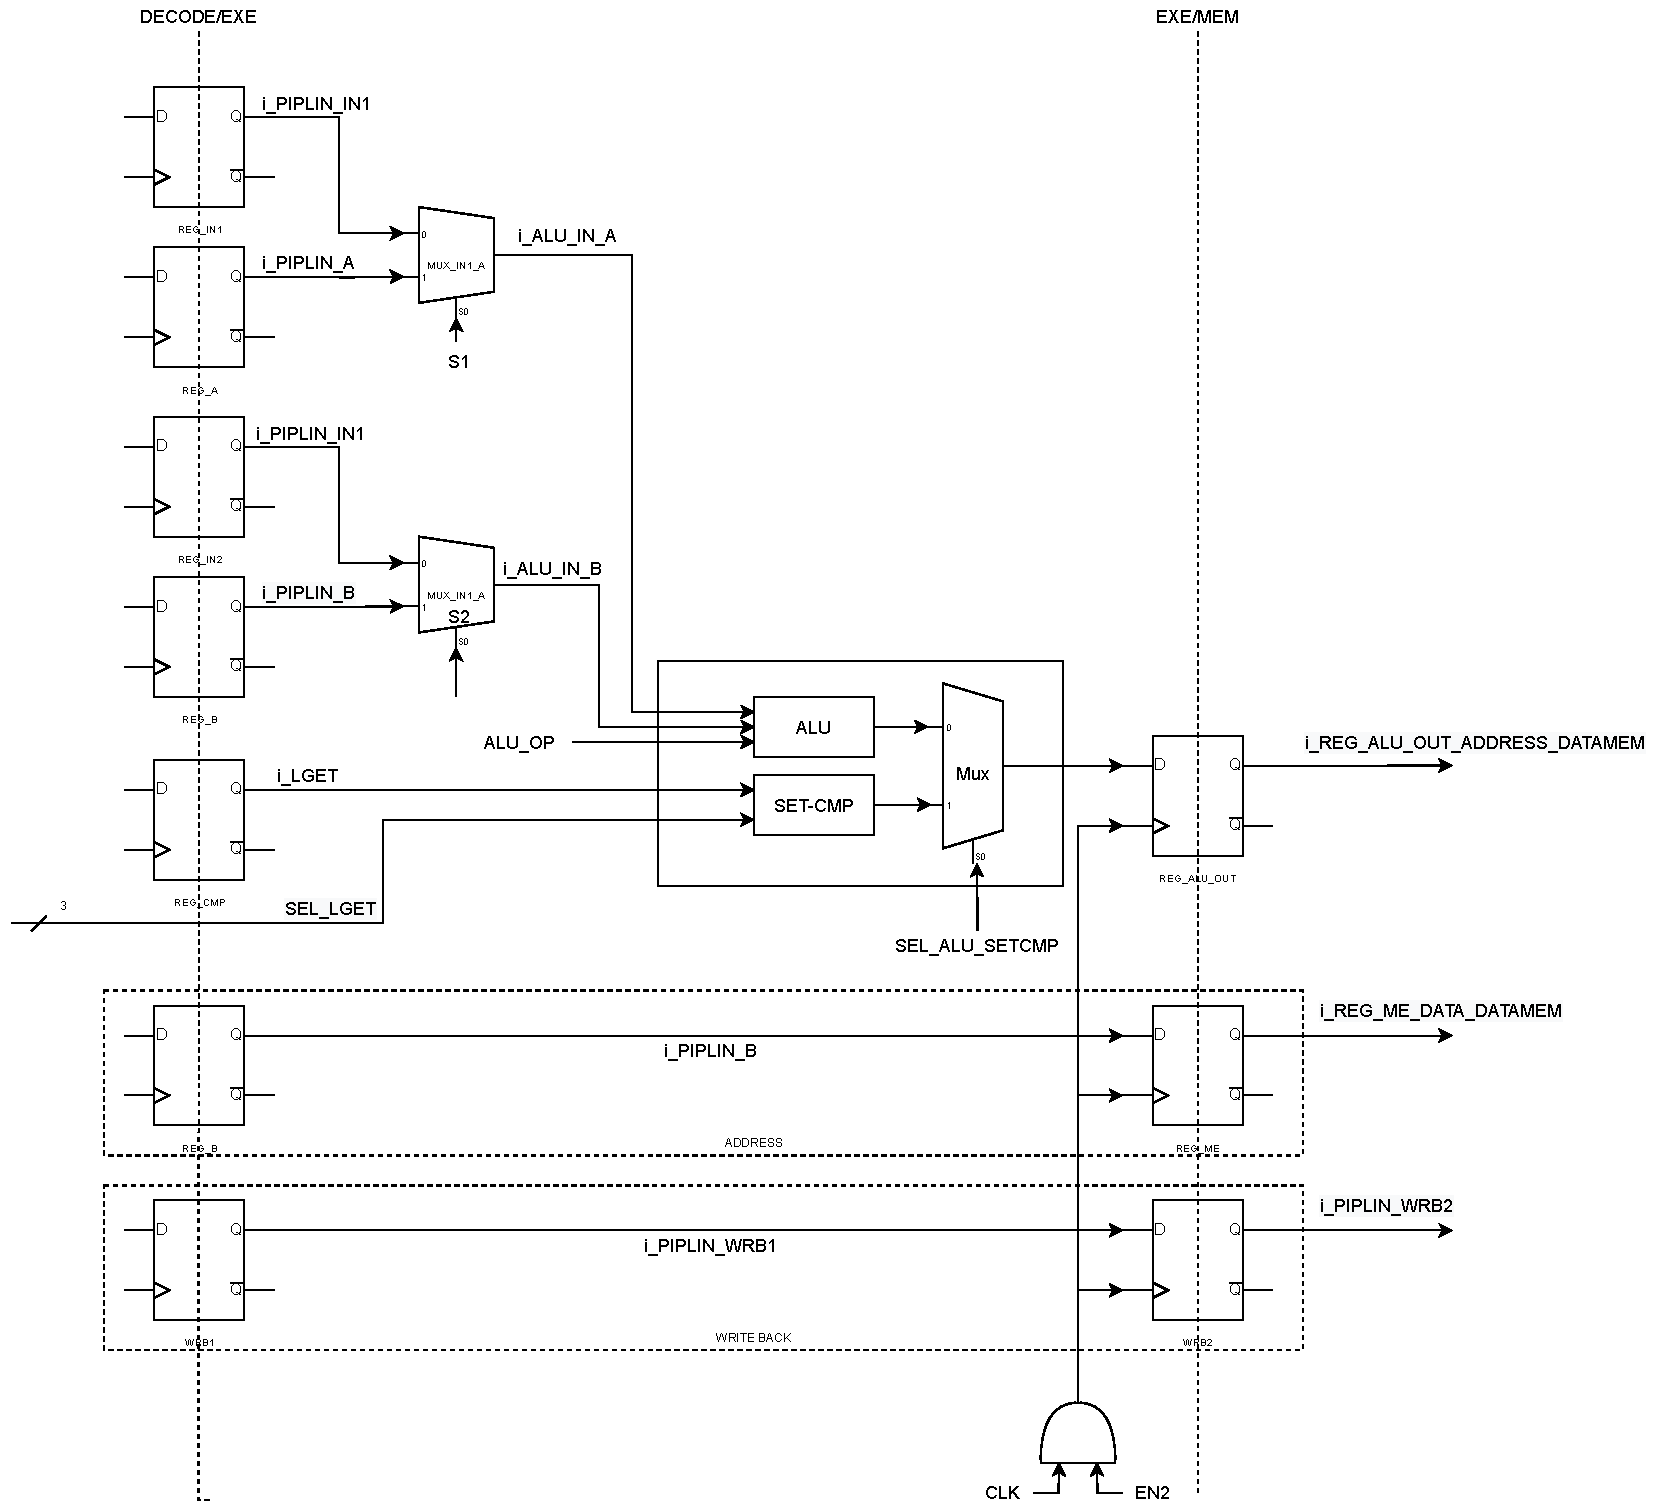
\includegraphics[width=0.9\textwidth]{chapters/5_ExecuteStage/images/exe_stage.pdf}
	\caption{Execute stage}
	\label{fig:execute-stage}
\end{figure}

The execute stage is the second stage of the Datapath and it is used to perform computation over data, like sum, multiplication, shift and logical operation; the Control Word coming from the Control Unit, allows to correctly configure the internal signal to perform the desired operation with the correct operands. In fact, in this stage we have multiple signals that can be configured:
\begin{itemize}
	\itemsep0sp
	\item \texttt{EN1}: this signal used in order to enable/disable the registers sampling in the DECODE/EXE junction;
	\item \texttt{EN2}: this signal used in order to enable/disable the registers sampling in the EXE/MEM junction;
	\item \texttt{S1}: this signal is used to select between the output of \texttt{REG\_A} (from register file) and \texttt{REG\_IN1} (immediate). If 0, \texttt{REG\_A} is selected;
	\item \texttt{S2}: this signal is used to select between the output of \texttt{REG\_B} (from register file) and \texttt{REG\_IN2} (immediate). If 0, \texttt{REG\_B} is selected;
	\item \texttt{SEL\_ALU\_SETCMP}: it is used to select the input for \texttt{REG\_ALU\_OUT} between the SET-CMP and ALU outputs;
	\item \texttt{SEL\_LGET}: this is a 3 bits signal, that is used to select among the \texttt{SEQ, SNE, SLE, SLT, SGE, SGT} operation for the SET-CMP unit;
 	\item \texttt{ALU\_OP}: this is a 5 bit signal, that is used to select the correct operation among the sub-unit that composes the ALU. Refer to the Table \ref{tab:alu_op} for a complete description.
	
\end{itemize}

Besides the main path, used to compute the output result, two addition paths (the ones in the dotted rectangles) are present in order to correctly manage the execution of all the operations in the instruction set:
\begin{itemize}
	\item A path for the propagation of the register value to be saved into the memory in case of a load. It was not possible to pass through the addition with \texttt{B} and \texttt{0} because it's already needed in order to compute the address. So, the output from \texttt{REG\_B} is directly connected to the input of \texttt{REG\_ME};
	\item The second path is the one used to manage the Write Back, at each step, until the MEM one, the reference to the register to perform the WB must be propagated through three stages (decode, execute and memory). So, the output of the \texttt{WRB1} register goes into the input of the \texttt{WRB2} register.
\end{itemize}

\section{ALU: Arithmetic Logic Unit}
\begin{figure}[h]
	\centering
	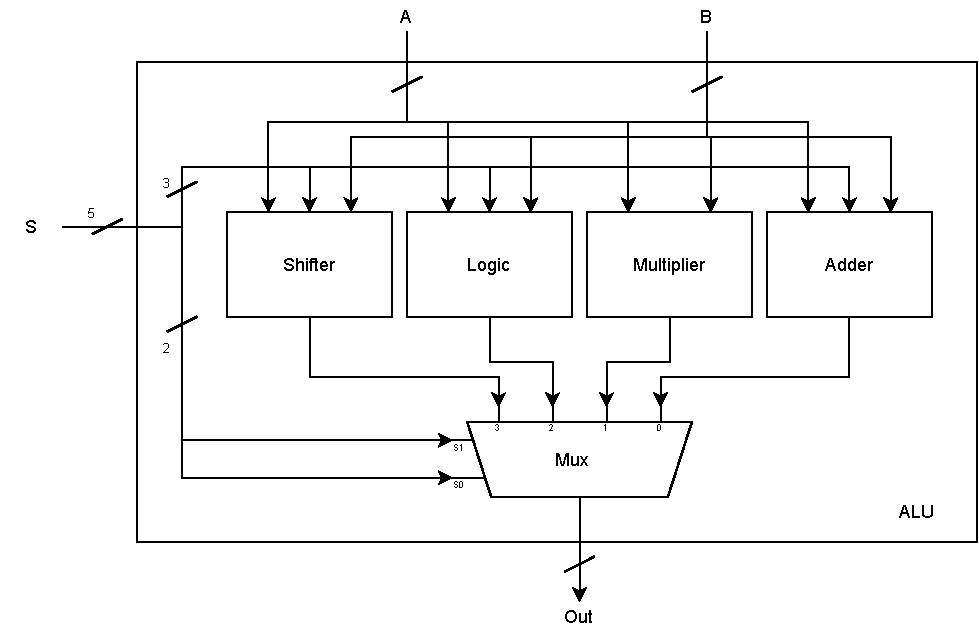
\includegraphics[width=0.6\textwidth]{chapters/5_ExecuteStage/images/ALU.pdf}
	\caption{ALU unit}
	\label{fig:ALU}	
\end{figure}
The Arithmetic Logic Unit can be seen as a block, that given a selection signal and the inputs is able to perform computation over the operands. The ALU implementation described in this document is based on the following block:
\begin{itemize}
	\itemsep0sp
	\item Adder
	\item Multiplier
	\item Logic unit
	\item Shifter
\end{itemize}
Each one of these blocks will be explained in the following sections.


The base concept is that, internally, the 4 units are selected through a multiplexer that takes two out five bits from a selection signal called \texttt{OP}. Having 5 bits to describe the type of operation, the possible combinations and their relative operations are:
\begin{table}[H]
	\centering
	\begin{tabular}{c | c |l}
		\texttt{OP} & \textbf{Unit} &\textbf{Operation}\\
		\hline
		000 00 & \multirow{2}{*}{ADD}& ADD\\
		001 00 & & SUB \\
		\hline
		000 01 & MUL & MUL\\
		\hline
		000 10 & \multirow{6}{*}{LOGIC}& AND \\
		001 10 & & NAND \\
		010 10 & & OR \\
		011 10 & & NOR \\
		100 10 & & XOR \\
		101 10 & & XNOR \\
		\hline
		000 11 &\multirow{6}{*}{SHIFT} & SHIFT RIGHT \\
		001 11 & & SHIFT LEFT \\
		010 110 & & ARITH SHIFT RIGHT \\
		011 11 &  & ARITH SHIFT LEFT\\
		100 11 &  & ROTATE RIGHT\\
		101 11 &  & ROTATE LEFT\\
	\end{tabular}
	\caption{ALU operations encoding}
	\label{tab:alu_op}
\end{table}

The two LSBs are the ones used as a selection input for the multiplexer that select from which ALU unit takes the result. In fact, they univocally define the unit to be used. The remaining three MSBs are used as input for the units that compose the ALU in order to select the correct operation.


\subsection{Adder}
The straightforward way to implement an adder is to use the Ripple Carry Adder structure, which is composed of $N-1$ Full Adder and one Half Adder (the first), where $N$ is the number of bits of the two operands. This solution is not optimal from a timing point of view due to the time needed to propagate the carry, which defines the critical path, that is the bottleneck. \newline\newline
Since the sum and the subtraction are two of the most common operations, the DLX includes an adder that is based on a CLA - Carry Look Ahead (Sparse Tree) and a Carry Select Like Adder. The complete structure can be seen in figure \ref{fig:P4}.

\begin{figure}[h]
	\centering
	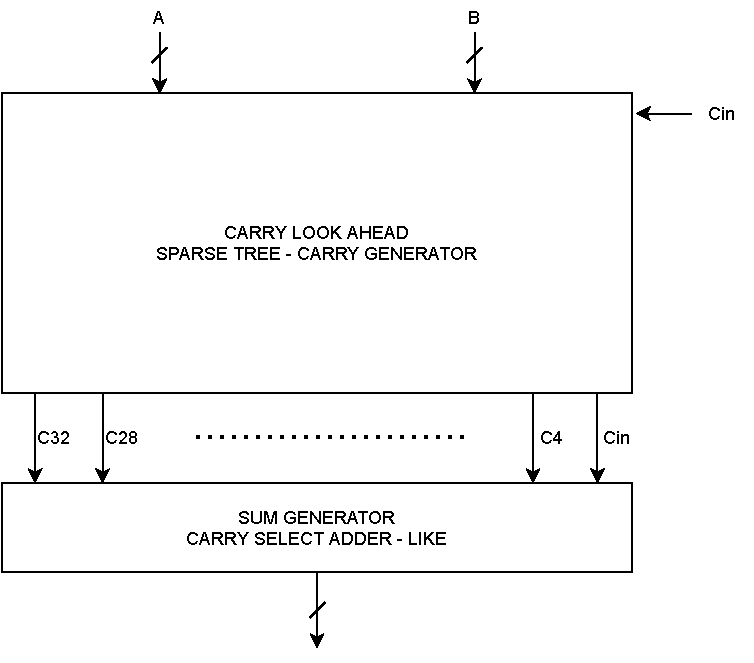
\includegraphics[width=0.5\textwidth]{chapters/5_ExecuteStage/images/P4.pdf}
	\caption{Booth's multiplier on 32 bits}
	\label{fig:P4}
\end{figure}
As said before, the adder is composed of two blocks:
\begin{itemize} 
	\item \textbf{Carry Select Like Adder}: The main point of the Carry Select Adder is that it doubles the complexity of the adder itself in order to obtain better performances. It is composed of two RCA to perform two sums in parallel.
	
	The idea is to compute both results, on 4 bits in this case, for both when the carry-in is equal to `0' or `1'. In this way, the results are computed in parallel for all the stages, even if the carry-in is `0' or `1'; then the carry-in is used to mux against the two results (on 4 bits) and the two carry-outs. The carry-out will be used as a result selection signal for the next Carry Select unit.
	
	We are paying complexity in order to reduce the sum computation time. In fact, by having a carry out that is used as carry in for the next state, there is still propagation but is lower.\newline\newline	
	The DLX implementation, instead of using a straightforward one of the Carry Select Adder, uses a modified version of it. It has been accomplished using \textit{CLA - Sparse Tree Carry Generator} and a \textit{Carry Select Like Adder}. The base idea is to use the CLA in order to compute a carry every $n$ bits; these carries are then fed into the sum generator that uses them to compute the results in parallel.
	\begin{figure}[H]
		\centering
		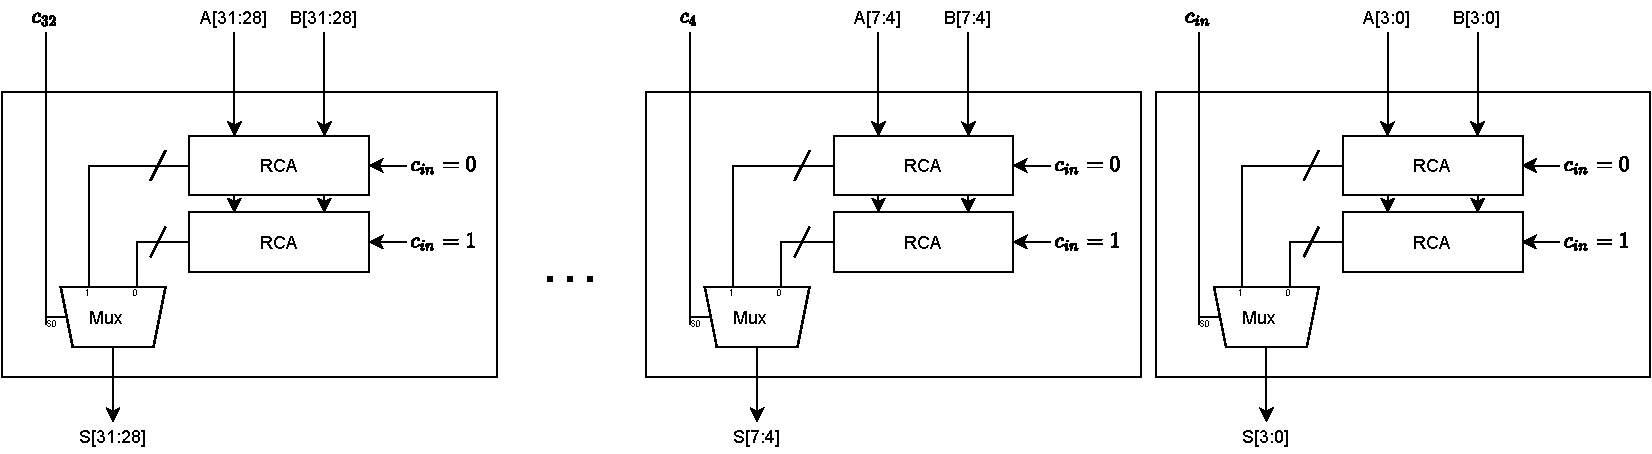
\includegraphics[width=1\textwidth]{chapters/5_ExecuteStage/images/carry_sum.pdf}
		\caption{Carry Select Like Adder block for a 32 bits implementation}
		\label{fig:carry_sum}
	\end{figure}
	\item \textbf{Carry Look Ahead - Sparse Tree}: this block is used to compute the carry out every 4 bits. The idea behind the CLA is to compute several carries simultaneously and to avoid waiting until the correct carry propagates from the stage of the adder in which it has been generated. This is done thanks to the \textit{propagate (P)} (that is 1 if the carry-in is equal to the carry-out) and \textit{generate (G)} (that is one if carry-in is 0 and carry-out is 1).
	\begin{table}[H]
		\begin{center}
			\begin{tabular}{ c c c | c c | c c}
				$a$ & $b$ & $c_{in}$ & $out$ & $c_{out}$ & $p$ & $g$ \\
				\hline
				0 & 0 & 0 & 0 & 0 & 0 & 0\\ 
				0 & 0 & 1 & 1 & 0 & 0 & 0\\ 
				0 & 1 & 0 & 1 & 0 & 1 & 0\\ 
				0 & 1 & 1 & 0 & 1 & 1 & 0\\ 
				1 & 0 & 0 & 1 & 0 & 1 & 0\\ 
				1 & 0 & 1 & 0 & 1 & 1 & 0\\ 
				1 & 1 & 0 & 0 & 1 & 0 & 1\\ 
				1 & 1 & 1 & 1 & 1 & 0 & 1\\ 
			\end{tabular}
			\caption{Computation of propagate and generate bits}
		\end{center}
	\end{table}
	\begin{equation} \label{eq:pandg}
		g = a \oplus b \quad\quad p = a \cdot b
	\end{equation}
	The base idea is to write any $s_i$, that is the i-esim bit of the sum and $c_i$, the carry-out at $i$ index in function of $p$ and $g$.
	We now use $p$ and $g$ to express the same result:
	\begin{align*}
		& s_1 = a \oplus b \oplus c_{in} = p_1 \oplus c_0\\
		& c_1 = a \cdot b + a \cdot c + b \cdot c = a_1 \cdot b_1 + (a_1 + b_1) \cdot c_0 =  g_1 + p_1 \cdot c_0
	\end{align*}
	The crucial point is that it's possible to compute the carry at $i$ position only using the initial carry-in $c_{in}$ and $p$ and $g$ generate in the current and previous blocks. Tree are a family of Carry Look Ahead that differ for the carry-logic. They are based always on \textit{propagate} and \textit{generate}. We have that 	
	\begin{align*}
		& carry = g + p \cdot c_{in}\\
		& G_{i:j} = G_{i:k} + P_{i:k} \cdot G_{k-1:j}\\
		& P_{i:j} = P_{i:k} \cdot P_{k-1:j}
	\end{align*}
	where
	\begin{itemize}
		\itemsep0sp
		\item $i \ge k > j$
		\item $G_{x:x} = g_x$ and $P_{x:x} = p_x$
		\item $g_0 = C_{in}$
	\end{itemize}
	The white and grey blocks in the Sparse Tree block at \ref{fig:pg_network}, that are used in the \texttt{carry\_generator} block, are PG and G blocks.
	Normally two blocks are used, the first \textit{G} generates only $G_{i:j}$ and the other \textit{PG} both $G_{i:j}$ and $P_{i:j}$.
	\begin{figure}[h]
		\centering
		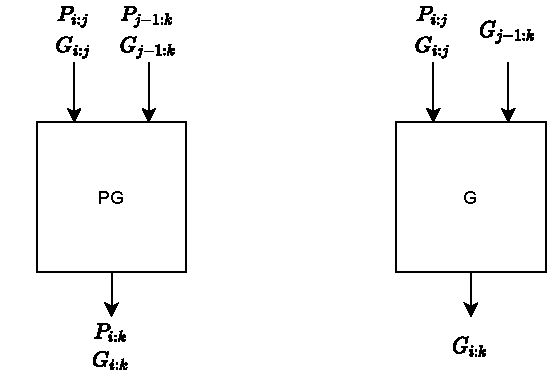
\includegraphics[width=0.32\textwidth]{chapters/5_ExecuteStage/images/PG_and_G.pdf}
		\caption{PG and P block}
		\label{fig:PG_and_G}
	\end{figure}
	The base idea is to combine their outputs and take only the G one as carries.
\end{itemize}
So, Carry Look Ahead - Sparse Tree needs a starting block that generates all the $p$ and $g$ for all the couples of bit using the \ref{eq:pandg} equation. The spars tree and the PG network structure is shown in the figure \ref{fig:pg_network}, in the code this block is called \texttt{prop\_gen\_generic} and is made of \texttt{prop\_gen} block in order to compute $p$ and $g$.
\begin{figure}[H]
	\centering
	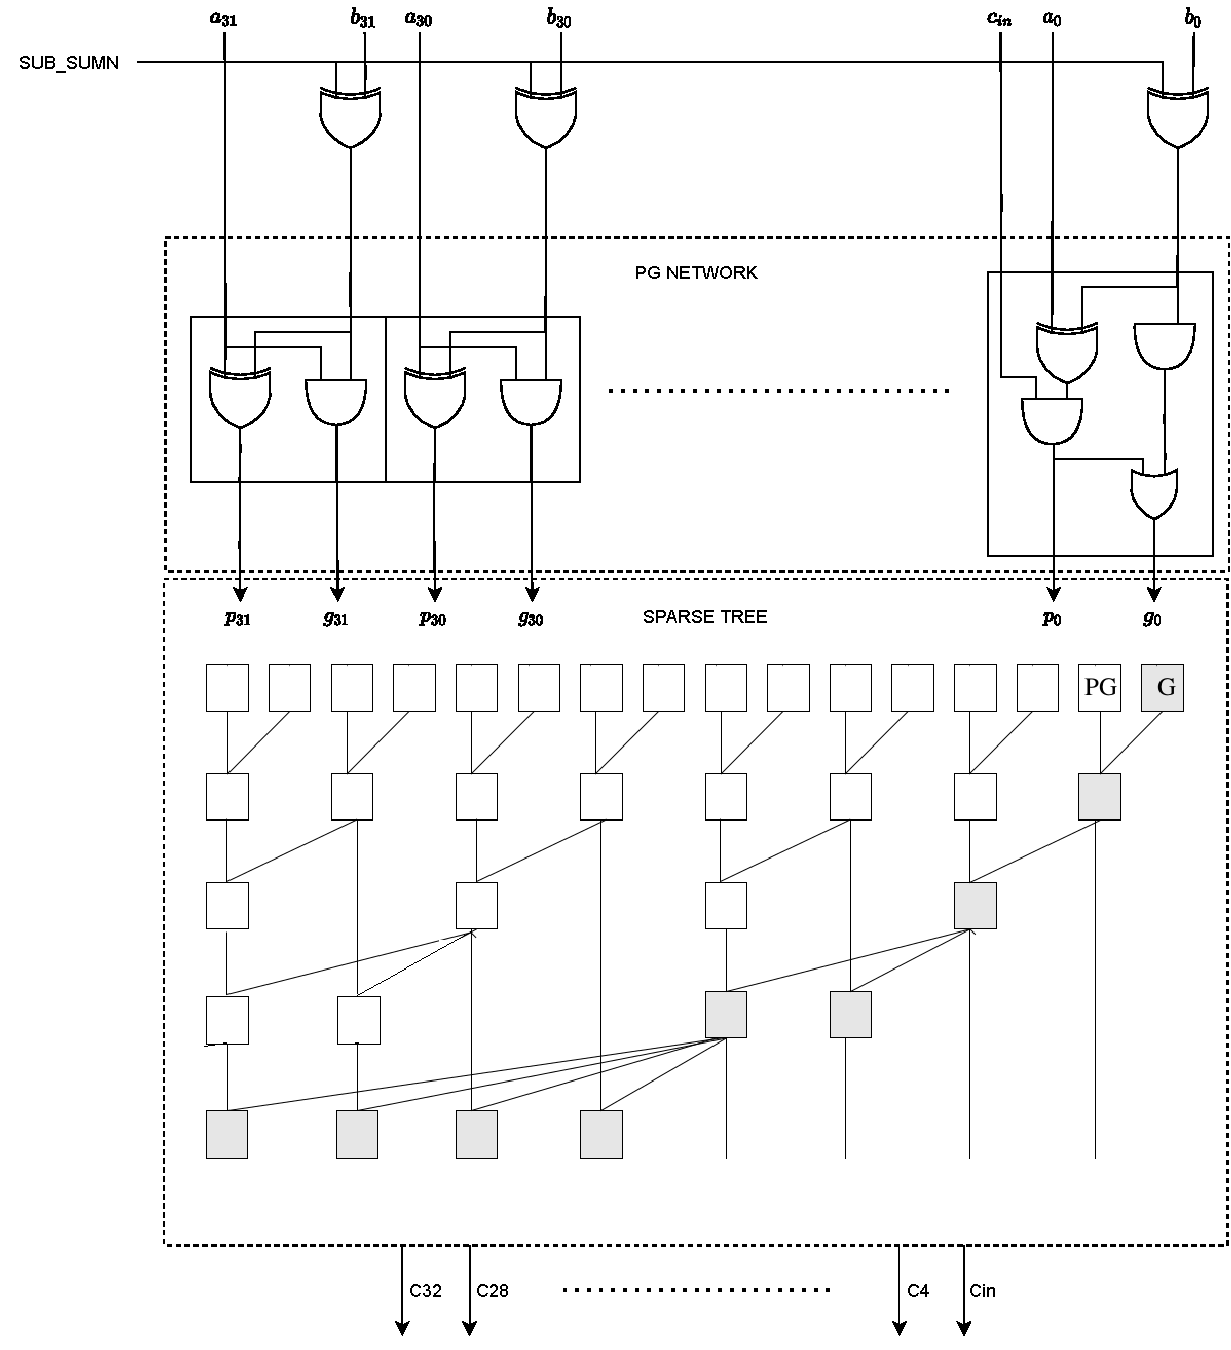
\includegraphics[width=0.65\textwidth]{chapters/5_ExecuteStage/images/CLA.pdf}
	\caption{Carry Look Ahead - Carry Generator Block}
	\label{fig:pg_network}
\end{figure}
To be able to perform both subtraction and sum, the first block must be modified and must include the logic to manage also the carry-in, that in case of subtraction is `1'. This is not enough to perform subtraction, in fact, an additional signal called \texttt{SUB\_SUMN} is needed.
The same structure can be used to implement subtraction by simply adding a XOR on each B input with the \texttt{SUB\_SUMN} control signal.

We can say that a subtraction in 2's complement can be implemented as $A + \overline{B} + 1$; in order to implement this in the circuit we need to set the carry-in to `1' (so \texttt{SUB\_SUMN} = `1') in order to add 1 and invert the B input by using the XOR. In fact:
\begin{displaymath}
	\begin{array}{c c|c}
		% |c c|c| means that there are three columns in the table and
		% a vertical bar '|' will be printed on the left and right borders,
		% and between the second and the third columns.
		% The letter 'c' means the value will be centered within the column,
		% letter 'l', left-aligned, and 'r', right-aligned.
		x & y & y \oplus q\\ % Use & to separate the columns
		\hline % Put a horizontal line between the table header and the rest.
		0 & 0 & 0\\
		0 & 1 & 1\\
		1 & 0 & 1\\
		1 & 1 & 0\\
	\end{array}
\end{displaymath}
This solution is good because the PG and G block has the same delay, that is driven by G and since both include it, they are the same. Many paths have the same delay and the load on components is good since an output of a block is connected to a maximum of 2 other blocks. These two factors bring a good \textit{equilibrium} to the entire structure.
\subsection{Multiplier}
In order to overcome the limitation of the array multiplier, this DLX implementation includes a modified version of the Booth's multiplier, since the multiplexer for the partial values to be added is only on two bits instead of three. The Booth's algorithm copes with 3 bits at a time, so the number of stages is $N/2$ (this corresponds to the number of the encoders) and this allows to speed up the result computation. 
The Booth's algorithm is the following:
\begin{lstlisting}[frame=none, escapeinside={(*}{*)}]
	i = 0
	P = 0
	while i (*$\leq$*) M - 2 loop
		P = P + Vp( (*$B_{i+1}, B_i, B_{i-1}$*) )
		A = A * 4
		i = i + 2
	end loop
\end{lstlisting}
Where \texttt{P} is the final value of the product and during the algorithm execution it will contain the partial result; \texttt{M} represents the number of bits of the multiplicand, in this case $B$. The algorithm takes as convention that $B_{i-1} = 0$. The \texttt{Vp} is a lookup Table (see \ref{mult:lut}), that return the value to add to \texttt{P}, according to the 3 bits selected. The value of $A$ is multiplied by 4.

\begin{table}[H]
	\begin{center}
		\begin{tabular}{ c c c | c}
			$B_{i+1}$ & $B_{i}$ & $B_{i-1}$ & \\
			\hline 
			0 & 0 & 0 & 0\\ 
			0 & 0 & 1 & +A\\ 
			0 & 1 & 0 & +A\\ 
			0 & 1 & 1 & +2A\\ 
			1 & 0 & 0 & -2A\\ 
			1 & 0 & 1 & -A\\ 
			1 & 1 & 0 & -A\\ 
			1 & 1 & 1 & 0\\ 
		\end{tabular}
		\caption{Booth's LUT}
		\label{mult:lut}
	\end{center}
\end{table}

The Booth's multiplier work with 3 main components, supposing $A$ is the multiplicand and $B$ the multiplier:
\begin{enumerate}
	\item $N/2$ encoders in order to take 3 bits from the operand $B$; the two LSB are used as a selection signals for the multiplexers and the last one, the MSB, for the adder. In fact, as shwon in Table \ref{mult:lut}, when the MSB is 1 the value to be added to the partial result is positive, negative otherwise. For this reason, the inputs of the multiplexers are only $\{0, A, 2A\}$. Since we also need to generate negative values, like ${-A, -2A}$, the MSB of the three bits is used as input for the adder. This signal, called \texttt{SUB\_SUMn} is used to define if the operation is a sum or a subtraction; if it is 1, a subtraction is performed;
	\item $N/2$ multiplexers that select only among $\{0, A, 2A\}$, since at each stage $A$ must be multiplied by 4, a shift by two is done starting from $A$ of the previous multiplexer;
	\item $N/2$ ripple carry adders, that allow to perform the partial sums. Since the final results will be on $NBIT \cdot 2+1$ bits, the adders in each level have been optimized in order to work only with the minimum bits needed. In fact, the adder at $i$ level, will generate the result on $NBIT + 2 \cdot i$ bits. As said before, a further signal called \texttt{SUB\_SUMn} has been added in order to be able to perform the subtraction. The Ripple Carry Adder has been selected for its simplicity and, since multiplication is a less common instruction, it was not worth using a more sophisticated adder. This allowed reducing the total area of the multiplier itself.
\end{enumerate}
The multiplexer implements the \textit{LUT} and at the same time the $A = A \cdot 4$. The two values from the two multiplexers are summed together via an adder, this implements the partial sum. The overall structure can be observed at \ref{fig:multiplier}.

\begin{figure}[ht]
	\centering
	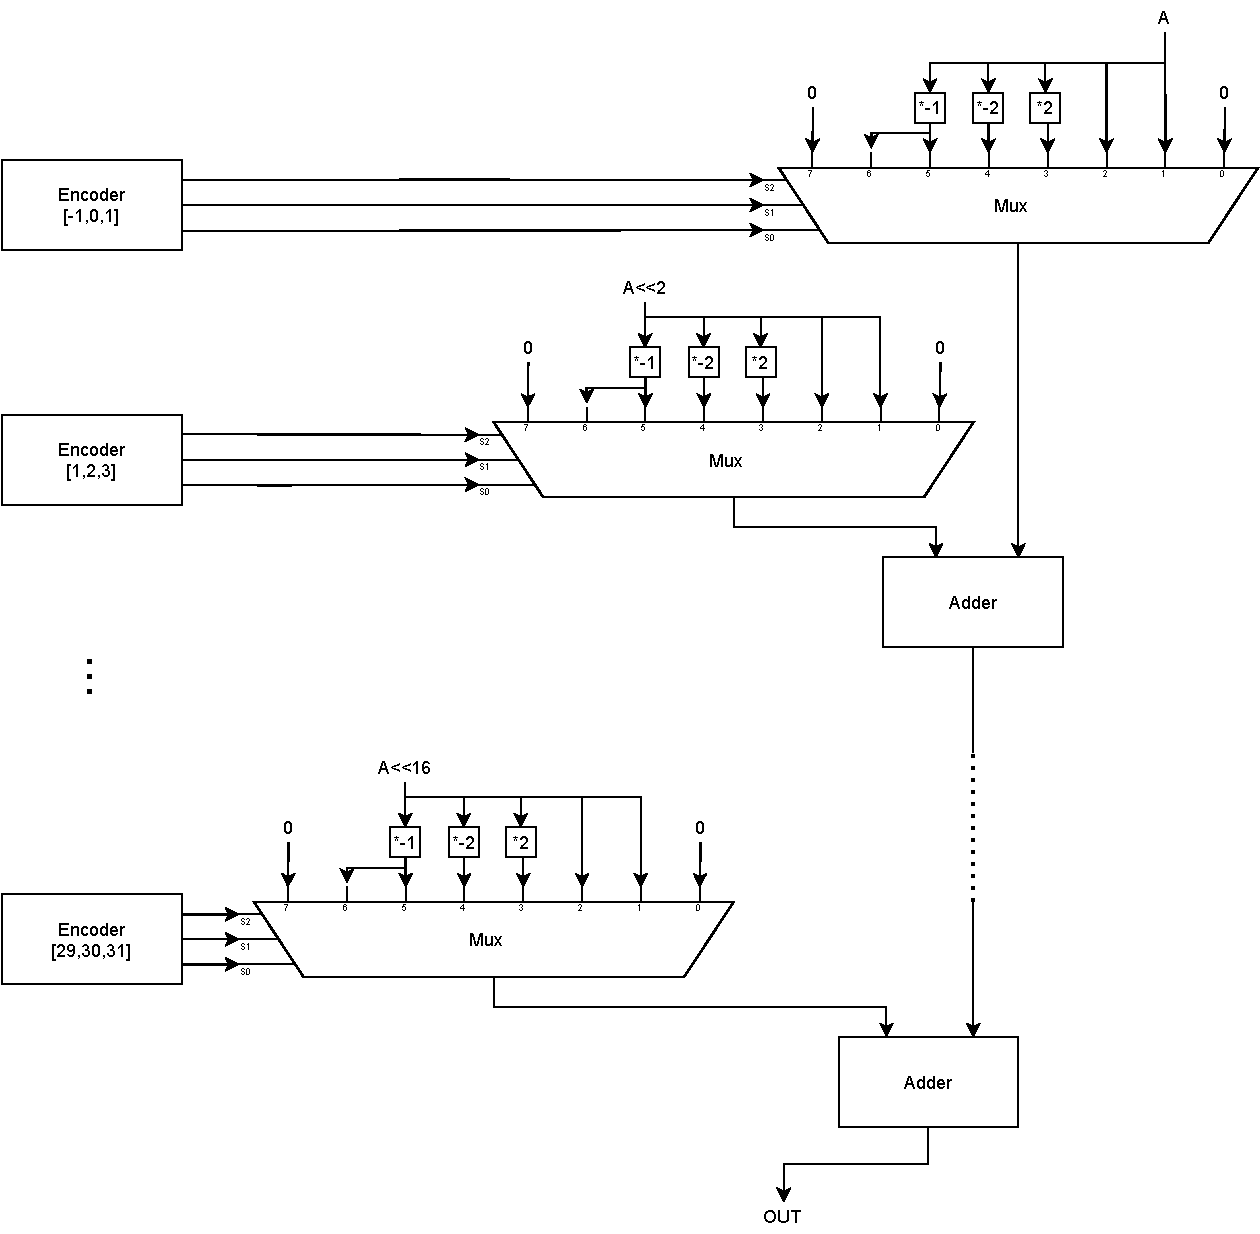
\includegraphics[width=0.8\textwidth]{chapters/5_ExecuteStage/images/multiplier.pdf}
	\caption{Booth's multiplier on 32 bits}
	\label{fig:multiplier}
\end{figure}

	
\subsection{Logic Operands}
The basic and most simple implementation of a logic unit is based on single logic gates on $N$ bits whose outputs are muxed, in order to generate the correct output. The problem with this solution is that the number of input signals of the multiplexer is extremely high; this implementation does not only suffer from a delay point of view but, since each logic function is implemented with a specific gate, also has a very high area usage.\newline\newline
In order to overcome the problems highlighted before, a more compact implementation has been chosen: the T2 logic unit.

This logic unit allows to perform AND, NAND, OR, NOR, XOR and XNOR using only 5 NAND gates, on two levels, and 4 selection signals. The schematic is the one in figure \ref{fig:log_unit}.

\begin{figure}
	\centering
	\tikzstyle{branch}=[fill,shape=circle,minimum size=3pt,inner sep=0pt]
	\begin{tikzpicture}[label distance=2mm]
		\draw (0.92,-0.40) -- (1.09,-0.56);
		\draw (1.92,-0.40) -- (2.09,-0.56);
		% nodes
		\node (y1) at (1,0) {$R_1$};
		\node (y2) at (2,0) {$R_2$};
		\node[not gate US, draw, rotate=-90] at ($(y1)+(0.5,-1.5)$) (noty1) {};
		\node[not gate US, draw, rotate=-90] at ($(y2)+(0.5,-1.5)$) (noty2) {};
		
		% draw nodes to NOT
		\foreach \i in {1,2} {
			\path (y\i) -- coordinate (punt\i) (y\i |- noty\i.input);
			\draw (punt\i) node[branch] {} -| (noty\i.input);
		}
	
		\node (x1) at (0,-2.33) {$S_0$};
		\node (x2) at (0,-3.33) {$S_1$};
		\node (x3) at (0,-4.33) {$S_2$};
		\node (x4) at (0,-5.33) {$S_3$};
		
		\node[nand gate US, draw, logic gate inputs=nnn] at ($(y2)+(2,-2.5)$) (And1) {};
		\node[nand gate US, draw, logic gate inputs=nnn] at ($(And1)+(0,-1)$) (And2) {};
		\node[nand gate US, draw, logic gate inputs=nnn] at ($(And2)+(0,-1)$) (And3) {};
		\node[nand gate US, draw, logic gate inputs=nnn] at ($(And3)+(0,-1)$) (And4) {};
		\node[nand gate US, draw, logic gate inputs=nnnn, anchor=input 1] at ($(And1.output -| And2.output)+(2,-1.25)$) (Or1) {};
		

		% connect x_i to AND_i
		\foreach \i in {1,2,3,4} {
			\draw (x\i) -- (And\i.input 1);
		}
		
		% y1

		\draw (noty1 |- And1.input 2) node[branch] {} -- (And1.input 2);
		\draw (noty1 |- And2.input 2) node[branch] {} -- (And2.input 2);
		\draw (y1 |- And3.input 2) node[branch] {} -- (And3.input 2);
		\draw (y1) |- (And4.input 2);
		\draw (noty1) |- (And2.input 2);
		
		\draw (noty2 |- And1.input 3) node[branch] {} -- (And1.input 3);
		\draw (y2 |- And2.input 3) node[branch] {} -- (And2.input 3);
		\draw (noty2 |- And3.input 3) node[branch] {} -- (And3.input 3);
		\draw (y2) |- (And4.input 3);
		\draw (noty2) |- (And3.input 3);
		

		% AND
		\draw (And1.output) -- ([xshift=0.8cm]And1.output) |- (Or1.input 1);
		\draw (And2.output) -- ([xshift=0.6cm]And2.output) |- (Or1.input 2);
		\draw (And3.output) -- ([xshift=0.6cm]And3.output) |- (Or1.input 3);
		\draw (And4.output) -- ([xshift=0.8cm]And4.output) |- (Or1.input 4);
	
		
		% OR
		\draw (Or1.output) -- ([xshift=0.5cm]Or1.output) node[above] {$out$};
		
	\end{tikzpicture}  
	\caption{Logic unit}
	\label{fig:log_unit}
	\end{figure}

	In order to compute one of the logical instructions, the select signals are properly activated as follow:
	
	\begin{figure}[ht]
		\centering
	\[
	\begin{vmatrix}
		S_0 & S_1 & S_2 & S_3 & \text{Operation}\\
		0 & 0 & 0 & 1 & AND \\
		1 & 1 & 1 & 0 & NAND \\
		0 & 1 & 1 & 1 & OR \\
		1 & 0 & 0 & 0 & NOR \\
		0 & 1 & 1 & 0 & XOR \\
		1 & 0 & 0 & 1 & NXOR \\
	\end{vmatrix}
	\]
	  \caption{Logic input signals with the relative operation}
	  \label{tab:log_sign}
\end{figure}
	
	For example, in order to generate the AND logical operation, we have to select $S_3 = 1$, so that $out = R_1 \cdot R_2$; on the other hand, if we need NAND $S_0 = S_1 = S_2 = 1$ and $S_3 = 0$, so that $out = \overline{R_1} \cdot \overline{R_2} + \overline{R_1} \cdot R_2 + R_1 \cdot \overline{R_2} = \overline{R_1} \cdot \overline{R_2}$ that using the De Morgan law $out = \overline{R_1 \cdot R_2}$.
	This allows to obtain the best performances also because all paths work in parallel, compacting the area and the delay.\newline\newline
	Since only the 3 bits are used to select among the logical operations (\texttt{S} signal), a direct correspondance is needed to generate the signal show in Table \ref{tab:log_sign}. The following table, shows the conversion:
	\begin{table}[H]
		\begin{center}
			\begin{tabular}{ c| c}
				\texttt{S} & Decoded signal \\
				\hline
				000 & 0001 \\
				001 & 1110 \\
				010 & 0111 \\
				011 & 1000 \\
				100 & 0110 \\ 
				101 & 1001 \\ 
				110 & 0000 \\ 
				
			\end{tabular}
			\caption{Conversion table, from \texttt{S} input signal on 3 bits into 4 bits}
		\end{center}
	\end{table}

\subsection{Shifter}
The implemented shifter allows to perform shift right, logical/arithmetical shift left and left/right rotate using the full operand \texttt{A} on 32 bits and 6 bits from the second one \texttt{B} and three \textit{control signals}.
Differently from the T2 version, it uses and addition signal in order to be able to manage also the rotate instruction. Our implementation takes three inputs:
\begin{itemize}
	\itemsep0sp
	\item \texttt{A}: the operand to be shifted/rotated;
	\item \texttt{B}: only the 5 LSB [4,3,2,1,0] are used to select first the mask to be used and then the starting point from that mask;
	\item \texttt{SEL}: it encodes the operation type; the second bit is used to select among arithmetic and logic, the third bit is used to select the direction of the shift/rotate (left/right) and the first one is used only if the operation is a rotate. This is the encoding:
	\begin{center}
		\begin{tabular}{c|l}
			\texttt{SEL} & \textbf{Operation}\\
			\hline
			000 & Shift logic right \\
			001 & Shift logic left \\
			010 & Shift arith right \\
			011 & Shift arith left \\
			100 & Rotate right \\
			101 & Shift right \\
		\end{tabular}
	\end{center}
\end{itemize}

\begin{figure}[ht]
	\centering
	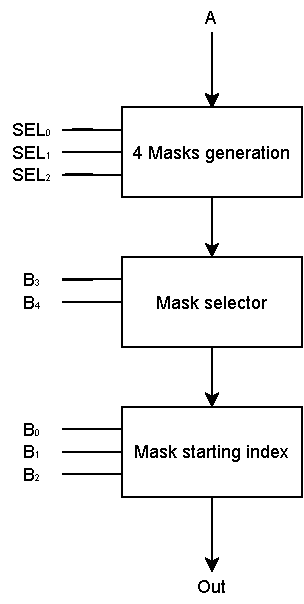
\includegraphics[width=0.2\textwidth]{chapters/5_ExecuteStage/images/Shifter.pdf}
	\caption{Blocks of the Shifter/Rotate Unit}
	\label{fig:shifter}
\end{figure}

 The unit performs the requested operation in three stages, sketched in figure \ref{fig:shifter}:
\begin{enumerate}
	\item The first consist in preparing 4 possible ``masks", each already shifted of {0, 8, 16, 32} left
	or right depending on the configuration. This allows to shift for all 32 bits. It copies the input \texttt{A} into the 4 masks that will be used by the next stage. Being on 32 bits, the generated masks are on $32+8=40$ bits. The only difference between this implementation and the T2 one, is that, in case of rotate, the additional 8 bits of the masks are filled with the corresponding 8 bits that are going ``out" during the rotation.
	
	\item The second level perform a coarse grain shift, that consist on selecting one mask among the 4 possible ones generated in the previous stage. This selection is done using the bits {4, 3} of \texttt{B}.
	\item The third level, using the bits {2, 1, 0} of \texttt{B} and the selected mask, performs a fine grain refinement. The 3 bits allow to select the starting index from the mask, granting a selection among 8 positions.
\end{enumerate}



\begin{figure}[h] 
	\label{ fig7} 
	\begin{minipage}[b]{0.5\linewidth}
		\centering
		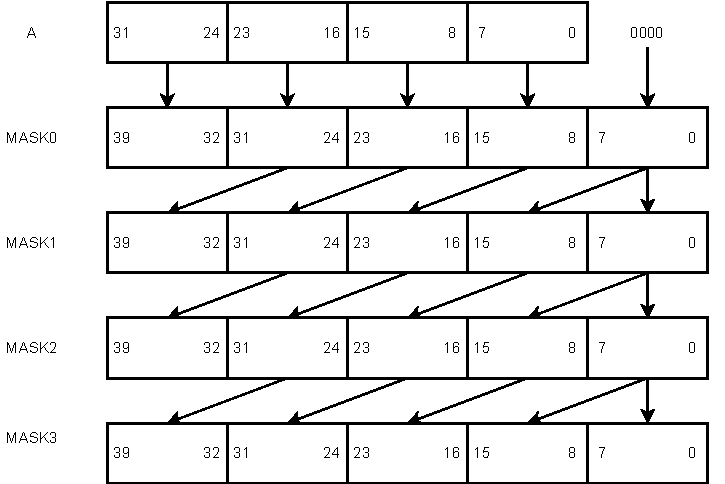
\includegraphics[width=.78\linewidth]{chapters/5_ExecuteStage/images/left_shift.pdf} 
		\caption{Masks for left shift} 
		\vspace{4ex}
	\end{minipage}%%
	\begin{minipage}[b]{0.5\linewidth}
		\centering
		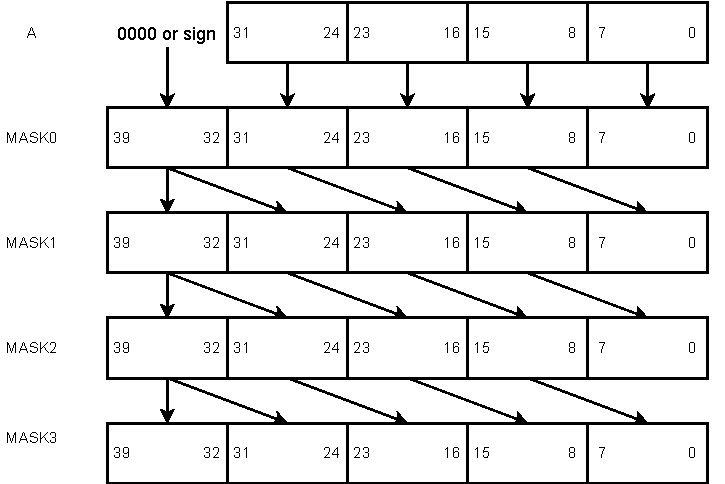
\includegraphics[width=.78\linewidth]{chapters/5_ExecuteStage/images/right_shift.pdf}
		\caption{Masks for right shift} 
		\vspace{4ex}
	\end{minipage} 
	\begin{minipage}[b]{0.5\linewidth}
		\centering
		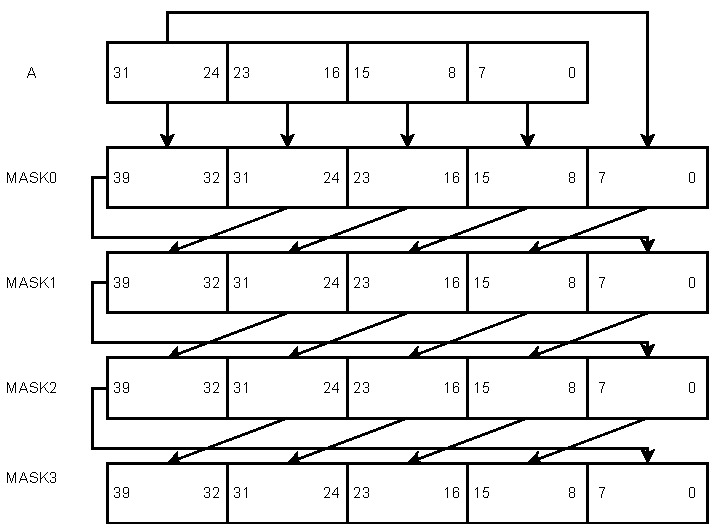
\includegraphics[width=.78\linewidth]{chapters/5_ExecuteStage/images/left_rotate.pdf} 
		\caption{Masks for left rotate} 
		\vspace{4ex}
	\end{minipage}%% 
	\begin{minipage}[b]{0.5\linewidth}
		\centering
		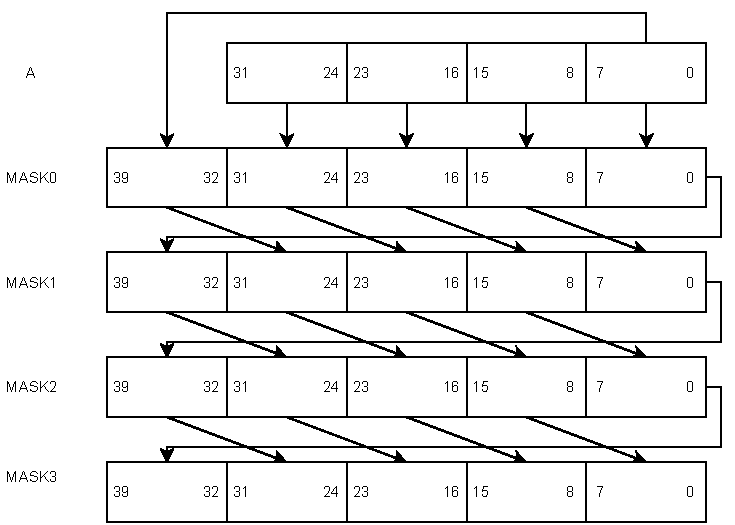
\includegraphics[width=.78\linewidth]{chapters/5_ExecuteStage/images/right_rotate.pdf} 
		\caption{Masks for right rotate} 
		\vspace{4ex}
	\end{minipage} 
	\caption{Masks for shift unit on 32 bits} 
\end{figure}
\begin{mybox}
	\textbf{Examples}
	\newline
	For example, if we need to perform a left left of 9 bits \texttt{A}, where \texttt{A=18}, the corresponding \texttt{B} value will be 1001; this means that the second masks will be taken and the output result will from the bit at position $40-1=39$ to the one at $39-32=7$ included.
	\begin{center}
		MASK 2: 0$\underbrace{\textbf{0000000 00000000 00000000 00010010 0}}_{\text{shifted \texttt{A}}}$0000000
	\end{center}
	
	On the other hand, if we need to perform a right shift the masks are generated in the opposite way, so the zeros are put in the MSB of the mask, shifted by 0, 8 ... positions. In this case there is also a distinction between the arithmetic and the logic shift; in the first case, instead of filling the ``empty" bits with zero, the operand sign is used. For example, if we want to shift \texttt{A=-18} of \texttt{B=3} bits, the first mask is used: 
	\begin{center}
		MASK 1: 11111$\underbrace{\textbf{111 11111111 11111111 11111111 11101}}_{\text{shifted \texttt{A}}}$110
	\end{center}
	
	In the last case, let's suppose to rotate right \texttt{A=1255} (=10011100111) by 5 position:
	\begin{center}
		MASK 1: 11$\underbrace{\textbf{100111 00000000 00000000 0000100 111}}_{\text{rotated \texttt{A}}}$00111
	\end{center}
	As you can see, in case of MASK 1 for the right rotation, the 8 LSB of \texttt{A} are copied into the 8 MSB of the mask.
\end{mybox}
	

\section{Set-Like Operations Unit}
\label{sec:set_like}
\begin{figure}[ht]
	\centering
	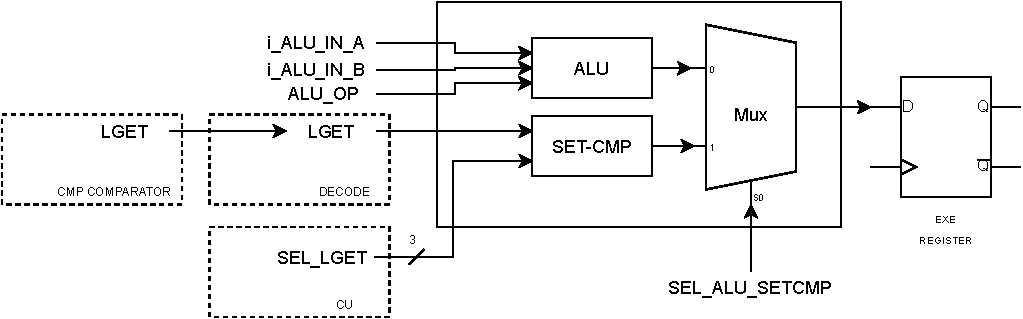
\includegraphics[width=0.8\textwidth]{chapters/5_ExecuteStage/images/set_cmp.pdf}
	\caption{Execute stage with focus on the SET-CMP unit}
	\label{fig:set-cmp}
\end{figure}

The DLX execution stage includes also the possibility to set the value of a register accordingly to the outcome of the comparison of two operands; the operands can came from two sources:
\begin{enumerate}
	\item Both from the register file, trough \texttt{REG\_B} and \texttt{REG\_A} (refer to figure \ref{fig:execute-stage});
	\item One from the register file (\texttt{REG\_A} by setting \texttt{S1 = 0}) and the immediate from \texttt{REG\_IN2} (refer to figure \ref{fig:execute-stage}).
\end{enumerate}

The unit designed to perform this set operation is called \texttt{set\_comparator}, that using a behavioural process, is able to generate the corresponding `1' or `0' to be set to the register, accordingly to the comparison result. The output on $N BIT_DATA$ bits will be muxed with the one coming from the ALU unit, using the CW that is configured in the Control Unit.

In order to decrease the area and since the comparison was already generated by the comparator unit in the decode stage (refer to section \ref{sec:comparator}), the \texttt{set\_comparator} unit takes the \texttt{LGET} signal that came from the decode unit and perform the following checks:

\begin{table}[H]
	\begin{center}
		\begin{tabular}{ c | l}
			\textbf{Operation} & \textbf{VHDL implementation} \\
			\hline
			\texttt{SEQ} & \texttt{not LGET(0)} \\
			\texttt{SNE} & \texttt{LGET(0)} \\
			\texttt{SLE} & \texttt{LGET(1) = `0' or LGET(0) = `0'} \\
			\texttt{SLT} & \texttt{LGET = "01"} \\
			\texttt{SGE} & \texttt{LGET(1) = `1' or LGET(0) = `0'} \\
			\texttt{SGT} & \texttt{LGET = "11"}
			
		\end{tabular}
		\caption{Performed checks in order to generate `1' or `0' accordingly to the comparison outcome. Refer to table \ref{tab:lget}.}
	\end{center}
\end{table}


